% LaTeX mintafájl szakdolgozat és diplomamunkáknak az
% SZTE Informatikai Tanszékcsoportja által megkövetelt
% formai követelményeinek megvalósításához
% Modosítva: 2011.04.28 Nemeth L. Zoltan
% A fájl használatához szükséges a magyar.ldf 2005/05/12 v1.5-ös vagy későbbi verziója
% ez letölthető a http://www.math.bme.hu/latex/ weblapról, a magyar nyelvű szedéshez
% Hasznos információk, linekek, LaTeX leírások a www.latex.lap.hu weboldalon vannak.
%

\documentclass[12pt]{report}

%Magyar nyelvi támogatás (Babel 3.7 vagy későbbi kell!)
\def\magyarOptions{defaults=hu-min}
\usepackage[magyar]{babel}

%Az ékezetes betűk használatához:
\usepackage{t1enc}% ékezetes szavak automatikus elválasztásához
\usepackage[utf8]{inputenc}% ékezetes szavak beviteléhez

% A formai kovetelmenyekben megkövetelt Times betűtípus használata:
\usepackage{times}

%Az AMS csomagjai
\usepackage{amsmath}
\usepackage{amssymb}
\usepackage{amsthm}

%A fejléc láblécek kialakításához:
\usepackage{fancyhdr}

%Természetesen további csomagok is használhatók,
%például ábrák beillesztéséhez a graphix és a psfrag,
%ha nincs rájuk szükség természetesen kihagyhatók.
\usepackage{graphicx}
\usepackage{psfrag}
\usepackage{stackengine,trimclip}

\usepackage{setspace}

\usepackage{hyperref}
\hypersetup{
    colorlinks,
    citecolor=black,
    filecolor=black,
    linkcolor=black,
    urlcolor=black
}

\usepackage{cite}

\usepackage{enumitem}
\usepackage{enumerate}

% Színek
\usepackage{color}
\definecolor{myCommentColorGreen}{RGB}{0,128,0}
\definecolor{myLineNumberGray}{RGB}{128,128,128}

% Forráskódhoz
\usepackage{listings}
\usepackage{lstautogobble}
\lstdefinelanguage{JavaScript}{
  keywords={break, case, catch, continue, debugger, default, delete, do, else, finally, for, function, if, in, instanceof, new, return, switch, this, throw, try, typeof, var, void, while, with},
  morecomment=[l]{//},
  morecomment=[s]{/*}{*/},
  morestring=[b]',
  morestring=[b]",
  sensitive=true
}
\lstset{ %
    %backgroundcolor=\color{white},   % choose the background color; you must add  \usepackage{color} or \usepackage{xcolor}
    basicstyle=\scriptsize, %\footnotesize,         % the size of the fonts that are used for    the code
    %breakatwhitespace=false,         % sets if automatic breaks should only      happen at whitespace
    breaklines=true,                  % sets automatic line breaking
    captionpos=b,                    % sets the caption-position to          bottom
    commentstyle=\color{myCommentColorGreen},    % comment style
    %deletekeywords={...},            % if you want to delete keywords              from the given language
    %escapeinside={\%*}{*)},          % if you want to add LaTeX                within your code
    %extendedchars=true,              % lets you use non-ASCII                  characters; for 8-bits encodings only, does not work with                  UTF-8
    frame=leftline,                   % adds a frame around the                    code
    %keepspaces=true,                 % keeps spaces in text,                      useful for keeping indentation of code (possibly needs                      columns=flexible)
    inputpath=../../../,
    keywordstyle=\color{blue},        % keyword style
    language=C++,                     % the language of                          the code
    literate=%
        {á}{{\'a}}1
        {é}{{\'e}}1
        {í}{{\'i}}1
        {ó}{{\'o}}1
        {ö}{{\"o}}1
        {ő}{{\H{o}}}1
        {ú}{{\'u}}1
        {ü}{{\"u}}1
        {ű}{{\H{u}}}1
        {Á}{{\'A}}1
        {É}{{\'E}}1
        {Í}{{\'I}}1
        {Ó}{{\'O}}1
        {Ö}{{\"O}}1
        {Ő}{{\H{O}}}1
        {Ú}{{\'U}}1
        {Ü}{{\"U}}1
        {Ű}{{\H{U}}}1,
    %morekeywords={*,...},            % if you want to                            add more keywords to the set
    numberfirstline=true,
    numbers=left,                     % where to put                              the line-numbers; possible values are (none, left, right)
    numbersep=10pt,                   % how far theline-numbers are from the code
    numberstyle=\tiny\color{myLineNumberGray}, % the stylethat is used for the line-numbers
    %name=\thelstnumber,              %
    %rulecolor=\color{black},         % if notset, the frame-color may be changed online-breaks within not-black text (e.g.comments (green here))
    showspaces=false,                % showspaces everywhere adding particularunderscores; it overrides'showstringspaces'
    showstringspaces=false,          % underline spaces within strings only
    showtabs=false,                  % show tabs within strings addingparticular underscores
    %stepnumber=2,                    % the step between two line-numbers.If it's 1, each line will benumbered
    %stringstyle=\color{mymauve},     % string literal style
    tabsize=4,                        % sets default tabsize to 2    spaces
    %title=\lstname                   % show the filename of     files included with     \lstinputlisting; also try     caption instead of title
}

% Kép mellett folyó íráshoz
\usepackage{wrapfig}

\usepackage[labelfont=it,justification=centering]{caption}

\usepackage{graphicx}
\usepackage{epigraph}
%\epigraphfontsize{\small\itshape}

%Tételszerű környezetek definiálhatók, ezek most fejezetenként együtt számozódnak, pl.
\newtheorem{tét}{Tétel}[chapter]
\newtheorem{defi}[tét]{Definíció}
\newtheorem{lemma}[tét]{Lemma}
\newtheorem{áll}[tét]{Állítás}
\newtheorem{köv}[tét]{Következmény}

%Ha a megjegyzések és a példak szövegét nem akarjuk dőlten szedni, akkor
%az alábbi parancs után kell őket definiální:
\theoremstyle{definition}
\newtheorem{megj}[tét]{Megjegyzés}
\newtheorem{pld}[tét]{Példa}

%%% Saját parancsok
% Az angol kifejezések kiemelése
\newcommand{\inenglish}[1]{\textsl{#1}}
\newcommand{\inenglishfn}[1]{\footnotesize{\inenglish{#1}}}
% A függvények a szövegben
\newcommand{\func}[1]{{\textsf{\footnotesize{#1}}}}

% A WRAPFIGUREnak adhatjuk meg az egész dolgozatban, hogy milyen globális
% stratégia szerint helyezze el a képeket: r - right, o - outside, l - left,
% i - inside, stb. A magyar makrónév melletti érv a lehetséges ütközések
% elkerülése. Az alapbeállítás az 'r', a szakdolgozat egyoldalas
% nyomtatása miatt, ha azonban az aktuális helyzet megkívánja, a makró
% használatát mellőzzük.
\newcommand{\melyikoldalra}{r}
%\newcommand{\melyikoldalra}{o} % az oldal külső felére

%\hyphenation{sza-bály el-kü-lö-ní-tett}

%Margók:
\hoffset -1in
\voffset -1in
\oddsidemargin 35mm
\textwidth 150mm
\topmargin 15mm
\headheight 10mm
\headsep 5mm
\textheight 237mm

\begin{document}


%%%%%%%%%%%%%%%%%%%%%%%%%%%%%%%%%%%%%%%%%%%%%%%%%%%%%%%%%%%%%%%%%%%%%%
%%   Címlap                                                         %%
%%%%%%%%%%%%%%%%%%%%%%%%%%%%%%%%%%%%%%%%%%%%%%%%%%%%%%%%%%%%%%%%%%%%%%

    %A FEJEZETEK KEZDŐOLDALAINAK FEJ ÉS LÁBLÉCE:
    %a plain oldalstílust kell átdefiniálni, hogy ott ne legyen fejléc:
    \fancypagestyle{plain}{%
    %ez mindent töröl:
    \fancyhf{}
    % a láblécbe jobboldalra kerüljön az oldalszám:
    \fancyhead[R]{\thepage}
    %elválasztó vonal sem kell:
    \renewcommand{\headrulewidth}{0pt}
    }

    %A TÖBBI OLDAL FEJ ÉS LÁBLÉCE:
    \pagestyle{fancy}
    \fancyhf{}
    \fancyhead[L]{\rightmark}
    \fancyhead[R]{\thepage}


    %A címoldalra se fej- se lábléc nem kell:
    \thispagestyle{empty}

    \begin{center}
    \vspace*{1cm}
    {\Large\bf Szegedi Tudományegyetem}

    \vspace{0.5cm}

    {\Large\bf Informatikai Tanszékcsoport}

    \vspace*{3.8cm}

    % Tíz sorral fentebb is át kell írni!!!
    {\LARGE\bf OpenGL-ES 2.0 alapú Path API}


    \vspace*{3.6cm}

    {\Large Diplomamunka}
    % vagy {\Large Szakdolgozat}

    \vspace*{4cm}

    %Értelemszerűen megváltoztatandó:
    {\large
    \begin{tabular}{c@{\hspace{4cm}}c}
    \emph{Készítette:}     &\emph{Témavezető:}\\
    \bf{Ledán Szilárd}  &\bf{Dr. Kiss Ákos}\\
    informatika szakos     &egyetemi adjunktus\\
    hallgató &
    \end{tabular}
    }

    \vspace*{2.3cm}

    {\Large
    Szeged
    \\
    \vspace{2mm}
    2018
    }
    \end{center}


    % 1.5-ös sorköz:
    % ezt javasolják:  \linespread{1.25}
    % és ez bevált, de ehhez kellett a \usepackage{setspace} csomag betöltése.
    \onehalfspacing


%%%%%%%%%%%%%%%%%%%%%%%%%%%%%%%%%%%%%%%%%%%%%%%%%%%%%%%%%%%%%%%%%%%%%%
%%   Mottó                                                          %%
%%%%%%%%%%%%%%%%%%%%%%%%%%%%%%%%%%%%%%%%%%%%%%%%%%%%%%%%%%%%%%%%%%%%%%

    \clearpage
    \thispagestyle{empty}
    {
    \setlength\epigraphrule{0pt}
    \linespread{1.0}\epigraph{\small\emph{,,A világ csak híd, menj át rajta,
    de ne építs rajta házat.''}}{\small(IHS)}
    }


%%%%%%%%%%%%%%%%%%%%%%%%%%%%%%%%%%%%%%%%%%%%%%%%%%%%%%%%%%%%%%%%%%%%%%
%%   Tartalomjegyzék                                                %%
%%%%%%%%%%%%%%%%%%%%%%%%%%%%%%%%%%%%%%%%%%%%%%%%%%%%%%%%%%%%%%%%%%%%%%

    \tableofcontents


%%%%%%%%%%%%%%%%%%%%%%%%%%%%%%%%%%%%%%%%%%%%%%%%%%%%%%%%%%%%%%%%%%%%%%
%%   Feladatkiírás                                                  %%
%%%%%%%%%%%%%%%%%%%%%%%%%%%%%%%%%%%%%%%%%%%%%%%%%%%%%%%%%%%%%%%%%%%%%%


    %A \chapter* parancs nem ad a fejezetnek sorszámot
    \chapter*{Feladatkiírás}
    %A tartalomjegyzékben mégis szerepeltetni kell, mint szakasz(section) szerepeljen:
    \addcontentsline{toc}{section}{Feladatkiírás}

A témavezető által megfogalmazott feladatkiírás. Önálló oldalon szerepel.


%%%%%%%%%%%%%%%%%%%%%%%%%%%%%%%%%%%%%%%%%%%%%%%%%%%%%%%%%%%%%%%%%%%%%%
%%   Tartalmi összefoglaló                                          %%
%%%%%%%%%%%%%%%%%%%%%%%%%%%%%%%%%%%%%%%%%%%%%%%%%%%%%%%%%%%%%%%%%%%%%%

    \chapter*{Tartalmi összefoglaló}
    \addcontentsline{toc}{section}{Tartalmi összefoglaló}

%A tartalmi összefoglalónak tartalmaznia kell (rövid, legfeljebb egy oldalas, összefüggő megfogalmazásban)
%a következőket: a téma megnevezése, a megadott feladat megfogalmazása - a feladatkiíráshoz viszonyítva-,
%a megoldási mód, az alkalmazott eszközök, módszerek, az elért eredmények, kulcsszavak (4-6 darab).

%Az összefoglaló nyelvének meg kell egyeznie a dolgozat nyelvével. Ha a dolgozat idegen nyelven készül,
%magyar nyelvű tartalmi összefoglaló készítése is kötelező (külön lapon), melynek terjedelmét a TVSZ szabályozza.

    \subsubsection*{A téma megnevezése}

A \emph{World Wide Web Consortium} (W3C) által \emph{Canvas 2D Context} néven
2015-ben elfogadott ajánlás \emph{path} részének megvalósítása \emph{OpenGL~ES~2.0} alapokon.

    \subsubsection*{A megadott feladat megfogalmazása}

Az előbb említett \emph{Canvas 2D Context} egy grafikus interfész. Ez az
interfész több grafikus függvényt definiál. Jelen dolgozat témája ezek közül az
úgynevezett \emph{path} részének leprogramozása úgy, hogy a lehető legtöbb
feladatot a grafikus processzor (\textit{GPU}) lássa el.

    \subsubsection*{A megoldásmód}

Több megoldás közül mi az alakzatok trapézokra bontását választottuk. Minden
trapéz felbontható további két háromszögre, amely megkötésre a OpenGL~ES~2.0
grafikus meghajtó miatt van szükség.

    \subsubsection*{Alkalmazott eszközök, módszerek}

Az API \emph{C++11} programozási nyelven készült, használva a következő
eszközöket, technológiákat: \emph{gcc}, \emph{git}, \textit{OpenGL~ES~2.0},
\emph{\LaTeX},

    \subsubsection*{Elért eredmények}

    \subsubsection*{Kulcsszavak}

grafika, path, Canvas 2D Context, OpenGL-ES 2.0


%%%%%%%%%%%%%%%%%%%%%%%%%%%%%%%%%%%%%%%%%%%%%%%%%%%%%%%%%%%%%%%%%%%%%%
%%   Bevezetés                                                      %%
%%%%%%%%%%%%%%%%%%%%%%%%%%%%%%%%%%%%%%%%%%%%%%%%%%%%%%%%%%%%%%%%%%%%%%

    \chapter*{Bevezetés}
    \label{Bevezetés}
    \addcontentsline{toc}{section}{Bevezetés}

A környezetünkben található számítástechnikai eszközök legtöbbjének van
grafikus kijelzője, és ezen eszközök mindegyike használ valamilyen
megjelenítő~\footnote{A számítógépes grafikában egy modell megjelenítését végző
folyamatot \emph{renderelés}nek (\inenglishfn{rendering}), a renderelést végző
programrészt pedig \emph{motor}nak (\inenglishfn{engine}) hívnak} (a
továbbiakban renderelő) függvénykönyvtárat. Ilyen például a Skia, a Cairo, az
OpenGL, és ilyen kíván lenni a \emph{Gepard} is. A cél egy \emph{C++11}-es
nyelven írt és több (\mbox{OpenGL~ES~2.0 \cite{Munshi:2008:OEP:1481069}},
Vulkan) grafikus renderelő motort támogató függvénykönyvtár.

A tervek szerint idővel a Gepard több interfésszel is rendelkezik. Így alkot
majd egy komplex grafikus alkalmazásprogramozási felületet
(\inenglish{Application Programming Interface}, a továbbiakban API). Az elsőnek
választott ilyen ismertebb interfész amit támogatni kíván az a \emph{W3C} által
készített \emph{Canvas 2D Context}~\cite{Cabanier:14:HCC} előírás.

A \emph{Canvas 2D Context} (a továbbiakban \emph{Canvas}) előírás 2015-ös
kiadása több elkülönített részből állítja össze az API-t. Ezen részek egyike az
úgynevezett \emph{Path}. Az említett 2015-ös előírás az 5., 8. és 11.
fejezetekben részletezi a Path-szal szembeni elvárásokat. A Path maga a
definiált grafikus alakzatokhoz képest bonyolultabbak leírását biztosító
eszköz. A Háttér (\ref{Háttér}.) fejezetben részletesebben kifejtjük a path-t
építő eszköz lehetőségeit és szabályait. Itt most csak annyiban kell kitérjünk
rá, hogy alapvetően két nagyobb részből áll. A \emph{körvonalból}
(\inenglish{stroke}) és a \emph{kitöltésből} (\inenglish{fill}).

Jelen dolgozat az említett \emph{Path} rész megvalósítását kívánja bemutatni.
Azt, hogy milyen szabályoknak kellett megfelelni, illetve milyen lehetőségeket
biztosított a választott OpenGL~ES~2.0 (a továbbiakban GLES2) szabvány, és azt,
hogy hogyan alkot köztes réteget ezek között a Gepard Path-t rajzoló, renderelő
része.

Első körben nem volt cél a ,,leggyorsabban futó'' és ,,legkisebb méretű''
Path-t rajzoló API elkészítése. Célunk egy lehetséges megvalósítás megtalálása,
és ez alapján egy olyan eszköz megalkotása volt, amely képes a választott
előírás (Canvas) elvárásait teljesíteni.


%%%%%%%%%%%%%%%%%%%%%%%%%%%%%%%%%%%%%%%%%%%%%%%%%%%%%%%%%%%%%%%%%%%%%%
%%   Háttér                                                         %%
%%%%%%%%%%%%%%%%%%%%%%%%%%%%%%%%%%%%%%%%%%%%%%%%%%%%%%%%%%%%%%%%%%%%%%

    \chapter{Háttér}
    \label{Háttér}

Ez a fejezet mutatja be azokat a technológiákat és kihívásokat, amelyek keretet
szabtak a téma megvalósításának. Szót kell ejteni magáról a Canvas 2D Context
API\footnote{Az alkalmazásprogramozási felület/interfész (Application
Programming Interface) kifejezésre a továbbiakban mint \emph{API} hivatkozunk.}
előírásról, a GLES2 szabvány nyújtotta lehetőségekről, azokról a matematikai
módszerekről, amelyek biztosítják számunkra, hogy tetszőlegesen bonyolult --
szerencsénkre zárt -- alakzatok kitöltését helyesen elvégezhessük. Össze
kellett kapcsolni a választott GLES2 szabta megkötést~\footnote { Az OpenGL 2.0
legfeljebb háromszögeket rajzol. } a Canvas Path~API elvárásaival~\footnote {
Elvárás a tetszőleges számú körcikk, szakasz és Bézier görbe alkotta -- akár
önmetsző -- alakzat mérethelyes megjelenítése. }. Ehhez több lépésbeli
megközelítést (\inenglish{approximation}) alkalmaztunk. Ezekről a lépésekről is
érdemes lesz beszélni.

    \section[A Canvas előírás]{A W3C Canvas 2D Context előírás}
    \label{A Canvas előírás}

A Canvas API egy közel tíz éves, kiforrott technológia\footnote {A W3C első
HTML5 szabvány-vázlata:\\ \footnotesize{
\url{https://www.w3.org/TR/2008/WD-html5-20080122/\#the-2d}} }. Az előírás leír
egy felbontásfüggő rajzolóvásznat, amelyet jellemzően \emph{Canvas}-nek
neveznek. A Canvas definíció szerint nem más mint egy adott \emph{szélességgel}
és \emph{magassággal} meghatározott terület, ahova különböző alakzatokat,
képeket, szövegeket és egyéb nem dinamikus grafikai elemeket rakhatunk fel. Az
elemeket függvények segítségével rajzolhatjuk a vászonra, vagy pedig a
Canvas-hez tartozó \emph{context} gyűjti, és bizonyos parancsok
(pl.~\emph{fill}) esetén az addig összegyűjtött elemeket kirajzolja a megadott
sorrendben. Végül mindig egy \emph{kép} (\inenglish{image}) vagy még
pontosabban egy \emph{bit-térkép} (\inenglish{bitmap}) készül.

Az előíráson belül definiált Path API rész amúgy egy régebbi, elterjedt
alakzatszerkesztő eljáráson alapul. Az eljárás lényege, hogy bizonyos alap
eszközökkel definiálunk egy bonyolultabb formát. Ezt a folyamatot hívjuk
alakzat építésnek (\inenglish{shape/path building}). Az építés fázis után
különböző parancsokkal rajzolhatjuk ki a definiált alakzatot, akár kitöltve
(\emph{fill}), akár körvonalként (\emph{stroke}), de lehetőségünk van az adott
alakzattal kivágni (\emph{clip}) is a Canvas-en már meglévő képből.

A Canvas előír néhány megkötést. Ezekről látni fogjuk, hogy természetes
korlátok. Hiszen józan ésszel felfogható, hogy egy egyenes szakaszból definiált
alakzatra értelmetlen a kitöltés, azaz a fill parancsot meghívni. Hasonlóan nem
mond semmit a nulla vastagságú vonal a stroke parancs esetén. Érdekes
belegondolni abba is, hogy mi legyen egy definiált alakzat sorsa, ha már
kirajzoltuk. Vessük el, vagy tartsuk meg. A szabvány megalkotói -- amúgy
programozási szempontból jól indokolható módon -- a megtartás mellett
döntöttek. Így viszont az a fontos megkötés is megjelent, hogy mindig
egyértelműen jelezni kell, ha új alakzatot akarunk definiálni.

A W3C-féle Canvas felfogható egy állapotgépnek. Ami ebben a esetben azt
jelenti, hogy bizonyos beállítások (kitöltőszín, betűméret, vonalvastagság,
transzformációk, stb.) érvényben maradnak mindaddig, amíg meg nem változtatjuk
azokat. Ezt már az előbb említett felépített vonal esetén is érezhettük. Mint
később látni fogjuk, ez erősen megköti a kezünket, hogy milyen rajzoló program
is lehet a Gepard. Persze a Gepard idővel kibővülhet további
funkcionalitásokkal (pl. \emph{flush}, \emph{finish}, stb.), amik egy sokkal
kötetlenebb rajzoló eszközhöz vezethetnek.

Térjünk vissza egy kis példa erejéig a Path építéshez. Feltételezzük, hogy a
kedvünkre beállítottuk a rajzolás színét, a méreteket és minden szükséges módon
felkészítettük a vásznunkat, hogy arra felvigyük a kívánt alakzatot. Ez most
legyen egy háromszög, mint az egyik legegyszerűbb, ám a szabványban külön nem
definiált forma, ellentétben a téglalappal (\emph{rect}, \emph{fillRect},
\emph{strokeRect}).

  \begin{figure}[!htb]
    \hspace{0.1\textwidth}
    \minipage{0.5\textwidth}
      \centering
      \begin{lstlisting}[language=JavaScript, autogobble=true]
        var cv = document.getElementById("Canvas");
        var ctx = cv.getContext("2d");
        ctx.beginPath();
        ctx.moveTo(5, 0);
        ctx.lineTo(6, 9);
        ctx.lineTo(0, 3);
        ctx.closePath();  // felső sor
        ctx.fill();  // utolsó két oszlop
        ctx.stroke();  // első két oszlop
      \end{lstlisting}
    \endminipage
    \hfill
    \minipage{0.5\textwidth}
      \includegraphics[width=.5\textwidth]{img/built/triangle}
    \endminipage
    \caption{\label{triangles-code-and-image} Bezárt és nyitva hagyott
    alakzatok körvonalai és kitöltései }
  \end{figure}

A fenti ábrán (\ref{triangles-code-and-image}) látható egy kis példakód,
illetve ennek hat különböző eredménye. Az első sorban olyan alakzatokat látunk,
ahol a \emph{closePath} parancsot meghívtuk (hármoszög), a másodikban pedig nem
(V alak). Az első oszlopban a \emph{fill}-t, a harmadikban pedig a
\emph{stroke}-ot nem hívtuk meg. Az előírás~\cite{Cabanier:14:HCC} ugyanakkor
rendelkezik arról, hogy minden Path zárt alakzat kell legyen, így mindig
kitölthető is. Ezért lett a második sor utolsó két V-nek definiált alakzata
mégis kitöltött háromszög. Nézzük meg, hogy milyen konkrét eszközöket biztosít
az előírás.

Ebben a fejezetben nem térünk ki részletesen a teljes előírásra. A legfontosabb
rész a dolgozatunk témája a Path. Ugyanakkor a munkához szorosan kapcsolódott a
környezet megvalósítása is. Ezért érintőlegesen beszélnünk kell a rajzolás
kontextusáról (\inenglish{drawing context}), a színek és vonaltulajdonságok
beállításáról, valamint a transzformációkról. Ezek után térünk rá az előírás
Path-t definiáló részére.

A rajzolás környezete, vagyis a \emph{context} tartalmazza, hogy milyen
színekkel fogunk rajzolni, milyen betűtípussal és mérettel, de ez tartalmazza
az aktuális transzformációt és itt van elméletileg letárolva az aktuálisan
felépített alakzat (\inenglish{path}) is. A context-nek mindig van egy aktuális
állapota (\inenglish{state}). A Canvas rendelkezik arról, hogy az aktuális
állapotot egy verembe elmenthessük és visszaállíthassuk. Ez a tulajdonsága a
vászonnak megkönnyíti a transzformációk alkalmazását egy-egy alakzatra, vagy
képre, esetleg szövegre. Ugyanakkor az állapot elmentése nem érinti az épített
alakzatot. Vagyis nincs hatással a path-ra. A context mindig egy path-t
tartalmaz, határoz meg. Ha például egy ilyen alakzatot több különböző színnel
és helyen akarunk a vászonra rajzolni, de nem akarjuk elveszíteni az aktuális
állapot szín és koordináta beállításait, akkor egy mentés után könnyedén
módosíthatjuk az attribútumokat, és tolhatjuk el az alakzatot. Majd a
kirajzolások után visszaállíthatjuk az elmentett állapotot.

Minket két színbeállítás érint. Az egyik az alakzat kitöltésekor használt
\func{fillStyle} attribútum. A másik az alakzat körvonalának színét meghatározó
\func{strokeStyle} attribútum. Ezek az attribútumok nem csak színek lehetnek,
hanem például leírhatnak egy gradiens színezést is. Illetve nem csak néhány
névvel előre definiált színt (\func{red}, \func{green}, \func{blue} stb.)
adhatunk meg, hanem különböző színterekből csatornánként saját színt is
beállíthatunk. Ilyen például az \emph{RGBA} (\func{rgb(red, green, blue,
alpha)}) vagy az \emph{HSV} (\func{hsv(hue, saturation, value)}) színtér. Sőt,
lehetőségünk van használni a webes környezetekben megszokott úgynevezett
hexa-kódokat. Ekkor az RGB színtérből választhatunk, és kétféle mintát
használhatunk: a hosszabb \func{\#rrggbb}-t és a rövidebb \func{\#rgb}-t. A két
attribútum viselkedését a CSS ajánlás\footnote{link} írja le. A beállítást
szöveges (\func{string}) formában kell megadni, amit aztán értelmezni kell, és
aszerint megadni az értékeket. Később részletesen lesz szó arról, hogy
milyen módon oldottuk meg a hasonló viselkedést C++-os környezetben.

A színekhez hasonlóan az alakzat körvonalának tulajdonságát leíró
attribútumokat is szöveg formájában kell megadni. Itt viszont van egy kis
játéktér, mert az ajánlások ugyan szöveget várnak, de a számértéket
váró attribútumok esetében (pl. \func{lineWidth}) azért elfogadhatunk majd
ténylegesen szám típust is. Erről is lesz szó az alakzatépítés
működését leíró fejezetben.

    \section[GLES2 API]{Az OpenGL~ES~2.0 API}
    \label{GLES2 API}

Az OpenGL~ES~2.0 (GLES2) azaz az \emph{Open Graphics Library for Embeded System
2.0}-ás verziója a \emph{Khronos Group} által felügyelt grafikus
függvénykönyvtár.  Segítségével majdnem közvetlenül adhatunk parancsokat a
grafikus egységnek. Az API-t alapvetően 3D modellek megjelenítésére
használhatjuk. Viszont maga az OpenGL egy hatalmas, komplex függvénykönyvtár.
Kisebb, hordozható eszközök esetén nincs szükség ekkora komplexitásra. Részben
ezért is vezették be az ,,asztali'' OpenGL megrostálása és egyszerűsítése révén
az ES API verziókat. Az ES verziók közül a 2.0-ás lett a
legelterjedtebb\footnote{TODO: hivatkozas}.  Viszonylag szigorú megkötések és a
kevés számú függvény ellenére jól használható. Ettől a verziótól már lehetővé
vált a \emph{programozható grafikus végrehajtási modell}
(\inenglish{programmable graphics pipeline}). Ami azt jelenti, hogy a
végrehajtási sorrendbe ugyan nem lehet belenyúlni, de az egyes lépésekben futó
részek programozhatók.

Nézzük meg röviden a dolgozat szempontjából fontos GLES2 megkötéseit.

A használható primitív alakzatelemek geometriai típusuk szerint a következők:
\emph{pont}, \emph{szakasz} és \emph{háromszög}. Ezek közül kitöltésre effektív
csak a háromszöget használhatjuk. Három típusát engedi a szabvány:
\emph{háromszög}, \emph{háromszögszalag} (\inenglish{triangle strip}) és
\emph{háromszög-legyező} (\inenglish{triangle fan}). Tehát az egyik és a
számunkra legfontosabb megkötés az, hogy a megjeleníteni kívánt alakzatot
háromszögekre kell bontanunk.

Bármilyen megjelenítéshez írni kell legalább két programot, ami a grafikus
egységen fog lefutni. Az első program kódját adja meg az ún. \emph{vertex
shader}, a másodikét a \emph{fragment shader}.

    \section[Matematikai háttér]{Matematikai háttér}
    \label{Matematikai háttér}

Az előbbi részekben már ismertetett kényszer miatt leírom, hogy az egyik régi
megközelítést fogom kissé tágabban értelmezve használni. Így a következő
egymásra épülő és használt matematikai fogalmakkal kell megismerkedni.

    \subsection*{Pásztázó-egyenesek}
    \label{Pásztázó-egyenesek}

A \emph{pásztázó egyenesek módszere} (\inenglish{scan-line algorithm}) egy
grafikai algoritmus alakzatok kitöltésére, vagy pont tartalmazásának
eldöntésére.\footnote{Foley link}

Az algoritmus jól ismert a számítógépes ábrázolás területén. Egyszerű módszer,
ezért nagy vonalakban ismertetjük. Kifejezetten kiemelve azokat a tényezőket,
amelyek a dolgozat szempontjából fontosabbak.

Legyen az alakzatokat leíró elemek listája. Fontos, hogy mindig zárt
alakzatokról van szó, ha a módszert vizsgáljuk. Az egyszerűség kedvéért a
leírást végezzük síkban. Ugyanakkor belátható, hogy a módszer térben is
működne. Vegyük az alakzatokat leíró elemek koordinátáit. Válasszuk ki
valamelyik dimenziót (például az $y$-t). Keressük meg a választott dimenzió
mentén a koordináták közül a legkisebbet. Ezután válasszunk egy olyan pontot a
síkon aminek a választott dimenziójú értéke még ennél is kisebb. Indítsunk
pásztázó vonalakat minden irányba ebből a pontból. Ekkor lesznek olyan vonalak,
amelyek nem érintik semelyik alakzatot sem. Viszont lesznek olyanok amelyek
metszik valamelyik alakzatelemet. A metszések és azok sorrendje a pásztázó
egyenesen kulcsfontosságúak. Aszerint, hogy milyen kitöltési stratégiát
választunk, nyernek értelmet a metszéspontok.

Vegyük elsőnek a \emph{paritás szabályt} (\inenglish{even-odd fill rule}). A
kiindulási ponttól egészen az első metszéspontig a pásztázó egyenes által
érintett pontokat nem jelöljük. Az első metszésponttól a következőig minden
pontot jelölünk, majd megint nem jelöljük a rákövetkezőig, és így
tovább. Egy pont az alakzat része, ha meg van jelölve. A megjelölt pontok
összességének képe a kitöltött alakzatok képe.

A másik elterjedt a \emph{nem-zérus szabály} (\inenglish{non-zero fill
rule}). Ahhoz azonban, hogy ezt a szabályt alkalmazni tudjuk, ismernünk kell
az alkatokat leíró elemeknek az irányítását. Ez lehet például a definiálás
sorrendje szerinti, stb. Itt a kiindulási pontól minden pontot zérussal
jelölünk, majd az első metszéspontnál vesszük a pásztázó vonal és az
elem irányításának keresztszorzatát. Az előjel szerint az eddigi zérus
értékhez hozzáadunk vagy kivonunk egyet, és a következő metszéspontig
ezzel az értékkel jelöljük a pontokat. A következő metszéspontban
hasonlóan járunk el, és az addigi értéket szintén eggyel módosítjuk.
Egy pont az alakzat része, ha nem zérus. Minden nem zérus pont együttes
képe a kitöltött alakzatok képe.

Természetesen a számítógépes ábrázolásban nem egy pontból indítjuk a pásztázó
vonalakat. A raszterkép valamelyik oldalára merőlegesen minden pontsorhoz
rendelünk egy a végtelenből jövő pásztázó vonalat. Ezek a vonalak teljesen
ekvivalensek a geometriaiakkal. Viszont azzal a megkötéssel igaze ez, hogy a
raszterpontok megjelölésére olyan szabályt kell alkalmazni, hogy a nem
raszterpont-határra eső, és érintkező alakzatok pontjai ne jelöljék meg
ugyanazt a raszterpontot kétszer.

  \begin{description}[noitemsep]
    \item[Kulcsszavak] pásztázó egyenes, pásztázó sáv.
    \item[Becsült oldalszám] 1.
  \end{description}

    \subsection*{\emph{Bézier} görbe és a \emph{de Casteljau} felbontás}
    \label{Bézier görbe és a de Casteljau felbontás}

A \emph{Bézier} (vagy \emph{de Casteljau}) görbecsalád használatának története
összenőtt~\footnote{TODO: Foley oldalszámos hívatkozás} a számítógépes
grafikáéval. Nem véletlen, hogy a Canvas API előírja a másod- és harmadrendű
Bézier görbék használatát. A következőkben általánosan bemutatjuk a
Bézier görbéket és azok tulajdonságait. Megvizsgáljuk a de Casteljau felbontást,
és bemutatjuk néhány olyan előnyét, amely indokolja a használatát.

Az alábbiakban definiáljuk a Bézier-görbéket. A definícióban a ,,pont'' fogalmát
nem szűkítjük a síkra, ugyanakkor világos, hogy a dolgozat esetében elégséges
erre a speciális esetre gondolnunk.

\begin{defi}\label{Bézier}\cite[Kurusa]{Kurusa:1999:szamitogepes}
Legyen adott az ($n+1$)-darab $p_0,...,p_n$ pont. Ezeket Bézier, vagy kontroll
pontoknak, az általuk meghatározott poligont pedig kontroll poligonnak nevezzük.
Indukcióval definiáljuk a következő pontokat, minden $t \in [0,1], k \in
\{{0,1,2,...,n\}}$ és $i \in \{{0,1,2,...,n-k\}}$ esetére:
\[p^0_i(t)=p_i,\]
\[p^k_i(t):=(1-t)p^{k-1}_i(t) + tp^{k-1}_{i+1}(t).\]
Ekkor azt a görbét, amit a $p^n_0(t)$ pont leír, amint a $t$ végig fut a $[0,1]$
intervallumon, Bézier görbének nevezzük, és $B(t)$-vel jelöljük. A $p^k_i(t)$
pontokat de Casteljau pontoknak, az $n$ számot pedig a görbe rendjének hívjuk.
\end{defi}

  \begin{figure}[!htb]
  \psfrag{a}[b][B][0.9]{\emph{a.}}
  \psfrag{P0}[b][B][0.8]{\bf{$p_{0}$}}
  \psfrag{P1}[b][B][0.8]{\bf{$p_{1}$}}
  \psfrag{P2}[b][B][0.8]{\bf{$p_{2}$}}
  \psfrag{P3}[b][B][0.8]{\bf{$p_{3}$}}
  \psfrag{P01}[b][B][0.8]{\bf{$p_{0}^{1}$}}
  \psfrag{P02}[b][B][0.8]{\bf{$p_{0}^{2}$}}
  \psfrag{P11}[b][B][0.8]{\bf{$p_{1}^{1}$}}
  \psfrag{P12}[b][B][0.8]{\bf{$p_{1}^{2}$}}
  \psfrag{P21}[b][B][0.8]{\bf{$p_{2}^{1}$}}
  \psfrag{P03}[b][B][0.8]{\bf{$p_{0}^{3}$}}
  \psfrag{b}[b][B][0.9]{\emph{b.}}
  \psfrag{Q0}[b][B][0.8]{\bf{$p_{0}$}}
  \psfrag{Q1}[b][B][0.8]{\bf{$p_{1}$}}
  \psfrag{Q2}[b][B][0.8]{\bf{$p_{2}$}}
  \psfrag{Q01}[b][B][0.8]{\bf{$p_{0}^{1}$}}
  \psfrag{Q02}[b][B][0.8]{\bf{$p_{0}^{2}$}}
  \psfrag{Q11}[b][B][0.8]{\bf{$p_{1}^{1}$}}
    \centering
    \includegraphics[width=.95\textwidth]{img/built/beziers_eps}
    \caption{\label{beziers} Bézier görbék. Az \emph{a. ábra} harmadrendű, a
    \emph{b. ábra} másodrendű görbe képét, kontroll poligonját és de
    Casteljau pontjait mutatja.}
  \end{figure}

A definícióból következik néhány tulajdonság. Nézzük ezek közül a
számunkra legfontosabbakat\footnote{TODO: Bizonyítások a Kurusa könyvében,
oldalak}:
\begin{itemize}[noitemsep]
  \item a Bézier görbe mindig a kontroll poligon első pontjától ($t=0$)
  kezdődik, és az utolsó pontjánál ($t=1$) ér véget,
  \item a $k$-adik rendű kontroll poligon $t/(1-t)$-ad felosztása megadja a
  ($k-1$)-edik kontroll poligont, amit tovább osztva a $t/(1-t)$ aránnyal, s
  ezzel eggyel csökkentve a kontroll poligon oldalainak számát, végül már csak
  egy pontot kapunk, ami a Bézier görbe $t$ paraméteréhez tartozó pontja, és az
  eljárást pedig \emph{de Casteljau felbontásnak} neveztük
  (\emph{\ref{beziers}. ábra}),
  \item az elsőrendű Bézier görbe egy \emph{egyenes},
  \item a másodrendű Bézier görbe egy \emph{parabola} (\emph{\ref{beziers}.
  ábra b.} pontja),
  \item a Bézier görbe mindig a kontroll poligon konvex burkában van,
  \item a Bézier görbe az affin transzformációkra invariáns, azaz a görbe
  affin képe megegyezik a kontroll poligon affin képe által meghatározott
  Bézier görbével.
\end{itemize}

A fenti tulajdonságokból is jól látszik, hogy miért lett népszerű a
számítógépes grafikában ez a görbecsalád.

A $t$ paraméterhez tartozó pont az $n$-ed rendű Bézier görbét két, ugyancsak
$n$-ed rendű görbére osztja. A két görbe kontroll pontjai pedig az eredeti görbe
de Casteljau pontjai közül kerülnek ki. A fenti tulajdonságokat és a
definícióban leírt indukciós elnevezést figyelembe véve a két $n$-ed rendű görbe
kontroll pontjai a következők:
\begin{equation}\label{eq:1}
B_{0\mapsto t}^n(t): p_0, p_0^1, ..., p_0^{n-1}, p_0^n; \qquad
B_{t\mapsto 1}^n(t): p_0^n, p_1^{n-1}, ..., p_{n-1}^1, p_n.
\end{equation}

\Aref{eq:1} felbontást később majd használni fogjuk. Világos, hogy a felbontást
tovább alkalmazva a görbe darabokon, végül a görbe darabok végpontjait sorban
összekötő egyenesek megközelítik az eredeti görbét.

  \begin{description}[noitemsep]
    \item[Kulcsszavak] Másod- és harmadrendű Bézier görbe, De
    Casteljau algoritmusa.
    \item[Becsült oldalszám] 2.
  \end{description}

    \subsection*{Körívek közelítése Bézier görbékkel}
    \label{}

Itt támaszkodunk egy cikkre, alapvetően annak a számunkra legfontosabb
tartalmát vesszük át.

  \begin{description}[noitemsep]
    \item[Kulcsszavak] Kör, körív.
    \item[Becsült oldalszám] 2.
  \end{description}


%%%%%%%%%%%%%%%%%%%%%%%%%%%%%%%%%%%%%%%%%%%%%%%%%%%%%%%%%%%%%%%%%%%%%%
%%   Alakzatrajzolás                                                %%
%%%%%%%%%%%%%%%%%%%%%%%%%%%%%%%%%%%%%%%%%%%%%%%%%%%%%%%%%%%%%%%%%%%%%%

    \chapter{Alakzatrajzolás}

A \emph{Gepard} tervezésekor fontos szempont volt, hogy ne csak az OpenGL
rajzoló modullal működjön. Vagyis lehetőséget kell kínálni, hogy a jövőben több
grafikus meghajtóval is tudjuk használni. Mint például a Vulkan, DirectX,
esetleg egy referencia szoftveres raszterizáló. Ezért a Gepard három részre
tagolódik (\ref{structure_eps}. ábra). A \emph{felső} réteg alapja a Canvas API.
Ezt neveztük el \emph{Gepard}-nak. A következő \emph{köztes} réteg fogja össze a
közös részeket. Ez lett a \emph{Gepard Engine}. A \emph{Gepard Backend} pedig az
\emph{alsó} szint, ahol az egyes grafikus meghajtók specifikus részei kaptak
helyet. Három modul fejlesztése történik itt: \emph{GLES2} (OpenGL ES 2.0),
\emph{Vulkan} (Vulkan 1.0) és \emph{Software} (saját raszterizáló).
  \begin{wrapfigure}{\melyikoldalra}{0.5\textwidth}
    \includegraphics[scale=0.45]{img/built/structure_eps}
    \caption{\label{structure_eps} A három fő réteg}
  \end{wrapfigure}
Ezeket a modulokat vagyis az ún. Backend-eket jelen pillanatban
\func{GepardEngineBackend} néven fordítási időben adjuk hozzá Gepardhoz, és
ezáltal a Gepard egy adott grafikus meghajtóra speciálisan lefordított
függvénykönyvtár lesz. Ugyanakkor a köztes (az Engine) és az alsó réteg
(valamelyik Backend) tervezéskori pontos szétválasztásának köszönhetően a
jövőben ez akár futás időben is megtörténhet. Javítva ezzel is az átjárhatóságot
a grafikus meghajtók között, és könnyebbé téve a Gepard használatát.

Most nézzük meg részletesebben a fent említett három réteget. Természetesen az
egyes rétegekhez kapcsolódó főbb részek, melyek tulajdonképpen a dolgozatunk
témája, külön fejezetben lesznek tárgyalva. Tehát most csak a rétegek
bemutatásához szükséges módon említjük meg ezeket.

    \subsection*{A felső réteg, azaz a Gepard interfész}

A felső réteget a \func{Gepard} osztályt \aref{Háttér}. fejezetben tárgyalt
Canvas határozza meg. Természetesen  a Canvas alapvetően egy webes interfész.
Ez azt is jelenti, hogy a \func{Gepard} nem teljesen úgy működik mint a Canvas
API a webes környezetben. A cél nem is az volt, hogy pontosan lemásoljuk. A cél
egy a C++ környezetben könnyen használható -- a webes szcénában már jól
kipróbált -- kezelőfelületet adjunk. Érdemes röviden átnézni ezt a felületet.

A Canvas API két csoportra osztható. Az egyik a hívható függvények, a másik a
beállítható adattagok csoportja. Tehát a Gepard interfész is többnyire ezt a
felosztást és működést próbálja meg követni. A hívható függvények tekintetében
egyszerűbb a helyzet. Hiszen az API által leírt függvények szemantikája nagyon
hasonló a C++ által elvártakhoz. A C++ környezet ugyan kissé megkötőbb. Például
szövegként (\inenglish{string}) átadott számértéket nem fogad el a szigorú
típusosság miatt. Ez azonban nem tekinthető durva megkötésnek, hiszen egyrészt
elemző-értelmező függvényekkel (\inenglish{parser functions}) az átváltások
biztosíthatók, és ugyanakkor az alap konverziók (\inenglish{cast}) továbbra is
működnek.

A függvények döntő része 32 bites lebegőpontos (\func{float}) vagy egész
(\func{int}) számot vár paraméterként. Ezért ezek könnyedén kezelhetők.
Ugyanakkor pár metódus esetében szükségszerű bevezetni saját típusokat,
osztályokat, struktúrákat, hogy a Canvas-hez hasonló viselkedést biztosíthassuk.
Ilyen osztály lett például az \func{Image}, amit többek között a
\func{putImageData()} függvény miatt kellett bevezetni. Szerencsére ezek az
osztályok is jól definiáltak a Canvas szintjén, vagyis szerkezetük jobbára
könnyen megadható.

A másik csoport a módosítható adattagoké (\inenglish{attributes}). Itt a
viselkedés kényelmes biztosításához saját osztályt kellett írni. Ez lett az
\func{Attribute} osztály. A bevezetésének szükségességét a \func{fillStyle}
adattagon keresztül mutatom be.

A \func{fillStyle} definíció szerint egy CSS attribútum\footnote{TODO: link
CSS-Style} vagyis adattag. Ez azt jelenti, hogy igen sokféleképpen lehet
értéket adni neki. A C++ szigorú típusossága miatt egyszerű, ún. primitív
típussal nem is megoldható, annak ellenére, hogy ez az adattag alapvetően csak
a kitöltés színét tárolja. Ugyanakkor a beállítás módja lehet hexa-kód
(\func{\#0f0} vagy \func{\#00ff00}), egy előre definiált név (\func{green}),
esetleg egy függvényszerű leírás vagy egy másik adattag értéke. Azáltal, hogy
az \func{Attribute} osztályt bevezettük, lehetőség nyílt az adattagok kényelmes
értékadásának.

Nézzük meg röviden ezt az osztályt is. Tehát mint már az előbb említettük
egyrészt, az értékadás sokféleségét biztosítani kellett. Ugyanakkor nem csak az
értékadás lehet többféle, hanem az adattagok ,,típusa'' is. Vagyis az említett
\func{fillStyle}-hoz képest más típusú adatot tároló módon is kellett tudjon
működni az \func{Attribute} osztály. Az értékadás sokféleségét egyrészt az
\emph{ad hoc polimorfizmus}\footnote{TODO:link!
https://www.itu.dk/courses/BPRD/E2009/fundamental-1967.pdf} biztosítja. A
bonyolultabb értékadásokat (pl. függvény leírás) pedig egy a példányosításkor
bekötött elemző-értelmező függvény végzi.
  \begin{wrapfigure}{\melyikoldalra}{0.3\textwidth}
  \begin{center}
    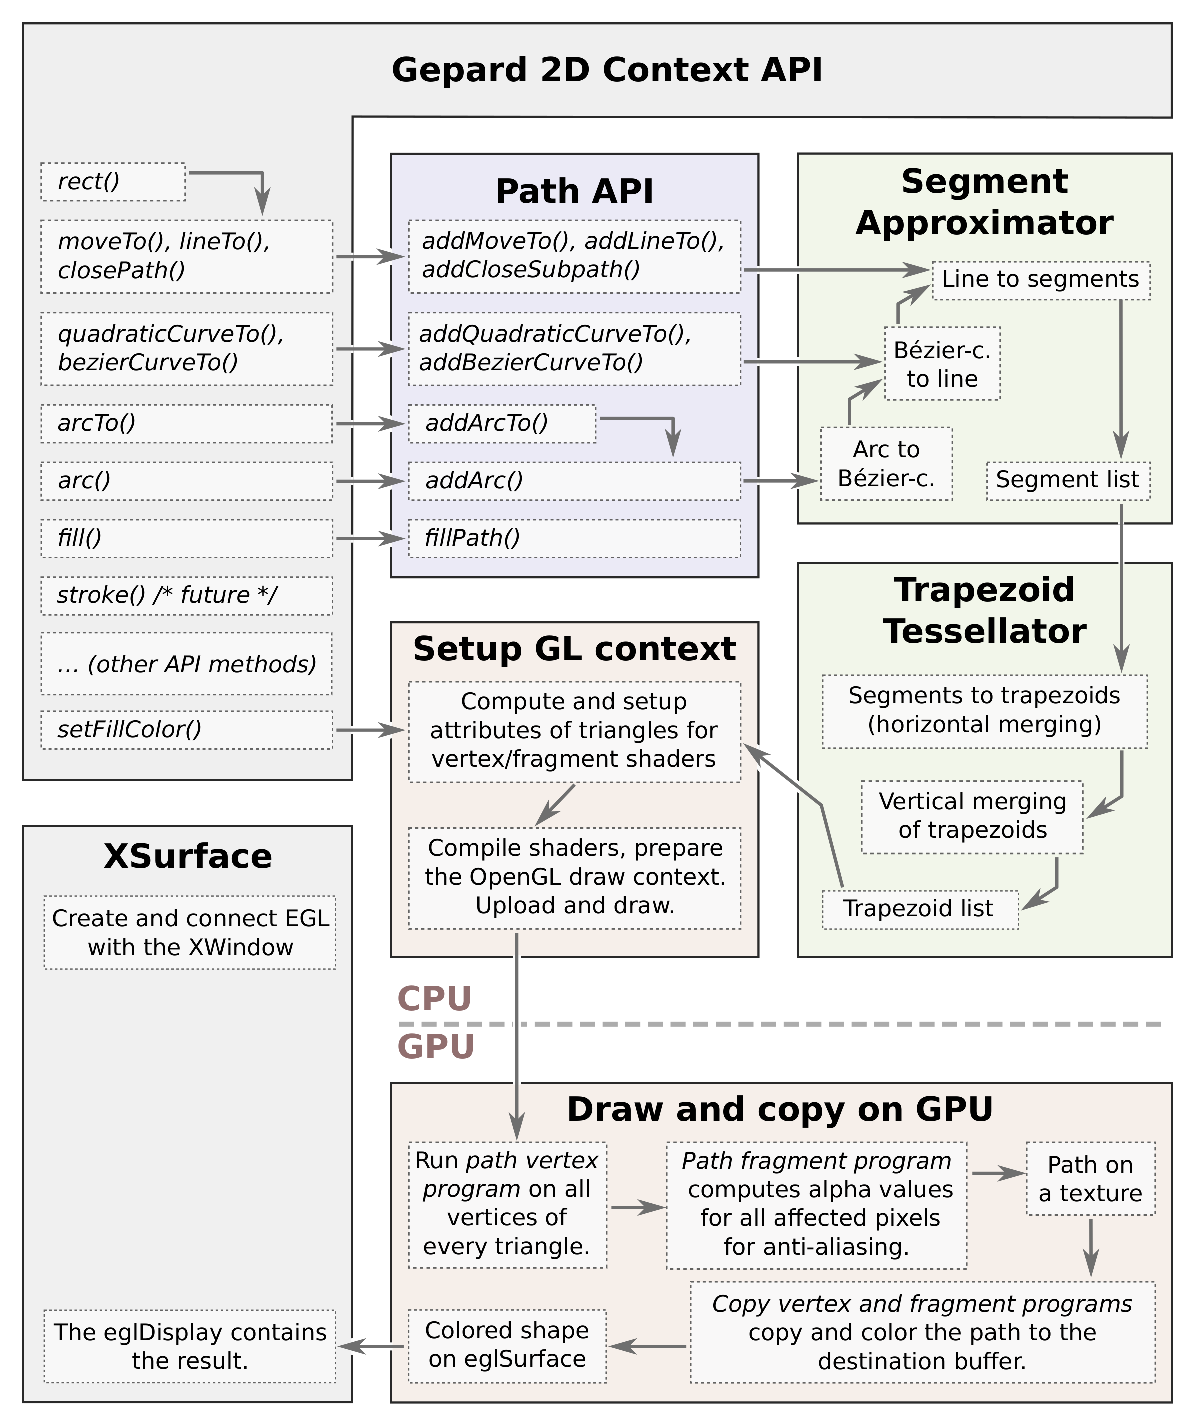
\includegraphics[scale=0.6,bb=0 210 160 590,
    clip=true]{img/built/dataflow_eps}
  \end{center}
    \caption{\label{dataflow-API-diagram} A \emph{felső} réteg, vagyis
    a Gepard interfész függvényei és adattagjai}
  \end{wrapfigure}
Az így bekötött függvény az értékadáskor meghívódik (visszahívódik,
\inenglish{callback}), és a kapott szöveget értelmezi, majd a megfelelő
adattagot immáron a középső rétegben vagyis a \func{Gepard Engine}-ben
beállítja.

\Aref{dataflow-API-diagram}. ábrán a Canvas API-nak a Geprad interfészben
általam megvalósított függvényei és adattagjai láthatók. A függvényeket a nevük
utáni zárójelpár jelzi. Az egyes függvények paramétereit itt nem tüntettük fel,
ezek úgy is megtalálhatók részletesebben is kifejtve az API dokumentációjában.
A zárójelpár nélküli nevek az egyes adattagok. Ezekről is tartalmaz bővebb
leírást a dokumentáció. A megvalósított API részek -- a gradiens színezést és a
szaggatott vonallal rajzolást leszámítva -- teljes körű alakzatrajzolást
biztosítanak számunkra. Erre láthatunk majd példát az eredményeket bemutató
fejezetben (\ref{Eredmények}). Az ábrán nem tüntettük fel a többi -- a
dolgozatot nem érintő API függvényt és adattagot.

Tehát az itt bemutatott \emph{felső} réteg vagyis a \func{Gepard} egy C++
interfész, ami egy jól bevált Canvas API-ra támaszkodik, és teremt kapcsolatot
a felhasználó és a következő ún. \emph{köztes} réteg között.

    \subsection*{A köztes réteg, azaz a GepardEngine osztály}

A köztes réteg már valamivel bonyolultabb. Egyrészt használja a grafikus
meghajtó specifikus alsóbb szintű réteget, előállítva a kívánt képet. Másrészt
tartalmazza és megvalósítja a közös osztályokat. Az egész réteget összefogó
osztály pedig a \func{GepardEngine}. Nézzük át részletesebben az itt
megvalósított részeket.

\Aref{structure_eps}. ábrán már láthattuk, hogy ez a szint a jelen dolgozatot
érintő négy főbb részből tevődik össze. Most csak hármat részletezünk itt. A
negyedik részt, azaz a \emph{Path} alakzatleíró és tároló és az ezt feldolgozó
osztályokkal úgy is külön alfejezetekben foglalkozunk.

Az egyik funkcionalitás a rajzolás környezetének (a továbbiakban kontextus,
\inenglish(drawing context))\footnote{\Aref{structure_eps}. ábrán ez az
,,Állapot kezelése'' rész.} biztosítása, bizonyos változások elmentése és
helyreállítása. Az elmentésért a \func{save}, a visszaállításért pedig a
\func{restore} API függvények a felelősek. A függvények hívásának hatásai ezen
a rétegen fejtődnek ki. A \func{save} egy verempufferbe teszi az aktuális
kontextus bizonyos beállításait. A \func{restore} pedig kiveszi a soron
következőt. Gyakorlatilag úgy kell értelmezni, hogy a verem tetején lévő
kontextus beállítások az érvényesek, azaz ezeket kell használni. Fontos
megjegyezni, hogy nem minden kontextusbeli elemet mentünk el, vagy állítunk
vissza. Például a transzformációkat, a kivágás alakzatát (\inenglish{clipping
region}) és a legtöbb színezéssel kapcsolatos értékeket igen, de a \emph{Path}
által aktuálisan tartalmazott alakzatot például nem. Itt csak a
legfontosabbakat soroltuk fel, de a Canvas API leírás \cite{Cabanier:14:HCC}
második fejezetében megtalálható a teljes lista.

A második rész a transzformációk. A Háttér részben (\ref{A Canvas előírás}) a
Canvas API bemutatásakor már tárgyaltuk\footnote{TODO: ellenőrizni!} a
transzformációkat, itt most csak röviden a megvalósításukat nézzük át.

Minden kontextus tartalmaz egy transzformációs mátrixot. Ezt a mátrixot a
\func{Transform} osztály valósítja meg. A megvalósítani kívánt mátrix egy
homogén sík koordinátás affin transzformációt tartalmaz. Aminek az alsó sora
ismert ($0\enskip 0\enskip 1$), így csak a felső két sort kell eltárolni. Ez
hat értéket jelent. Ebből a harmadik oszlopban találhatók a síkban eltolás
vektorának értékei. A hat lebegőpontos értéken kívül még megvalósítottuk a
leggyakrabban használt mátrix műveleteket, mint például a szorzás, inverz
számítás, stb.

Alakzatot rajzoló parancsok esetén a rajzolás pillanatában az aktuális
kontextus által tartalmazott mátrixot kell alkalmazni. Ez a primitív alakzatok
esetén könnyebb, hiszen az alakzat egyszerre definiálódik és rajzolódik ki.
Tehát a megfelelő koordinátákat megszorozzuk a transzformációs mátrixszal. A
\emph{Path} esetén figyelnünk kell arra, hogy az alakzat építése közben is
lehetséges a transzformációs mátrix módosítása. Ami azt jelenti, hogy az addig
épített alakzatra érvényesíteni kell a megváltoztatott mátrixot. Ugyanakkor az
alakzatot tovább lehet építeni. Az eltranszformált részt úgy kell felfogni,
mintha eredetileg is így eltranszformálva adták volna meg, vagyis
tulajdonképpen könnyedén folytathatjuk az alakzat építését.

Részben ehhez a réteghez kapcsolódik a kitöltött téglalap (\func{fillRect})
rajzolása is. Ez ugyan szigorúan nem tartozik a szakdolgozatunk tárgyához,
ugyanakkor mint a Path általános alakzatleírás egyik -- külön is definiált --
primitív alakzatként azért érdemes pár szót ejteni róla. Elsőre erre az
egyszerű alakzatra készült el a kirajzolás általános folyamata. Kezdve az API
hívástól (\func{fillRect}) a felső rétegben. Majd haladva a köztes rétegen át a
konkrét kirajzolásig OpenGL ES 2.0-t használva. A téglalapot mint két egymáshoz
illesztett derékszögű háromszöget értelmeztük. A négy sarokra mint vertexekre
hívódott meg egy nagyon egyszerű \emph{program} a grafikus eszközön. Az alakzat
egyszerűsége miatt mind a \emph{vertex}, mind pedig a \emph{fragment}
programrészekhez tartozó ún. árnyaló\footnote{FIXME: magyarul a shader?}
(\inenglish{shader}) kódok viszonylag egyszerűek lettek. Ezért könnyen
felállítható volt a rajzolás folyamata, ahová aztán be lehetett illeszteni a
komplexebb alakzatok megjelenítését.

    \section[A Path osztály]{A Path osztály}
    \label{A Path osztály}

A \func{Path} egy konténer osztály. A fő feladata, hogy az alakzatot és az
ahhoz szorosan kapcsolódó tulajdonságokat tárolja. Ebben a fejezetben ezt az
osztályt illetve a hozzá szorosan kapcsolódó kisebb struktúrákat fogjuk
bemutatni.

Az alakzat építéséhez tartozó kisebb struktúrák egyenként megfelelnek az API
szinten hívható path építő függvények valamelyikének. Vagyis a \func{moveTo}
híváshoz a \func{MoveToElement} struktúra tartozik és így tovább. A \func{Path}
osztályban minden elemhez tartozik egy függvény, amellyel ezekből a
struktúrákból adhatunk hozzá példányokat az épülő alakzathoz. Tehát a fenti
példában említett \func{moveTo} hatására a \func{Path}-beli \func{addMoveTo}
függvény hívódik, és hozzáad az alakzat építésének sorába egy példányt a
\func{MoveToElement} struktúrából. Természetesen nem minden alakzatépítő
híváshoz tartozik egyedi struktúra. Néhányat közülük visszavezethetünk egy vagy
több másikra. Ilyen például a \func{rect} API függvény, amit akár már a felső
rétegben is visszavezethetünk egy \func{moveTo} és három \func{lineTo} hívásra.
Vagy hasonló a \func{arcTo} API hívás. Ami ugyan meghívja a \func{Path} osztály
\func{addArcToElement} függvényét, ugyanakkor ez a függvény végül mégis csak
átalakítja ezt az elemet, és egy \func{LineToElement} valamint egy az
\func{arc} függvényhez tartozó \func{ArcElement} párosaként adja hozzá az
alakzatot leíró listához.

Minden speciális alakzatelemet definiáló struktúra egy közös ős
(\func{PathElement}) struktúrából származik. Tehát a megvalósított struktúrák a
következők:
  \begin{itemize}[noitemsep]
    \item \func{PathElement} (ős),
    \item \func{MoveToElement},
    \item \func{LineToElement},
    \item \func{CloseSubpathElement},
    \item \func{QuadraticCurveToElement},
    \item \func{BezierCurveToElement},
    \item \func{ArcElement}.
  \end{itemize}
Nézzük meg részletesebben ezeket a struktúrákat.

A \func{PathElement} mint ős definiálja a közös információkat. Minden
alakzatelemnek van végpontja, ahol az alakzatot rajzoló képzeletbeli tollhegy
megáll. Ez egy koordinátát tároló \func{to} adattag. Minden alakzatelemre igaz,
hogy vagy az utolsó, vagy követi egy újabb elem. A \func{next} adattag adja meg
a következő elem memóriacímét. Amennyiben ez \func{NULL}, az azt jelenti, hogy
az adott elem az utolsó struktúrája az alakzatnak. Minden struktúrának meg kell
tudnia mondania magáról, hogy a speciálisak közül melyik. Erre akkor van
szükség, hogyha ősként hivatkoznánk rá. Ezt adja meg a \func{type} adattag.

A \func{MoveToElement} jelöli az alakzatépítési-listában, hogy felemeltük a
tollat, és áthelyeztük egy másik pontba. A \func{LineToElement} egy egyenes
vonalat határoz meg az utolsó elem végpontjától a saját végpontjáig. A
\func{CloseSubpathElement} egy egyenes vonallal zárja a legutolsó
\func{MoveToElement} pontjából indított alakzatot. Mindhárom struktúra csak
annyiban tér el az őstől, hogy markerként hordozza a típusát.

A \func{QuadaraticCurveToElement} egy másodrendű Bézier görbét határoz meg az
előző elem végpontjától a saját végpontjáig az újabb adattagként megjelenő
kontrollpont szerint. A \func{BezierCurveToElement} egy harmadrendű
Bézier görbét határoz meg az előző elem végpontjától a saját végpontjáig a két
újabb adattagként megjelenő kontrollpontok szerint.

Az \func{ArcElement} struktúra leír egy körcikket. Ez a struktúra több
adattaggal is bővül az őshöz képest. Egyrészt tárolni kell a középpontot, a kör
sugarát, a körcikk kezdő és vég szögét, valamint a körbejárás irányát. Ezen
kívül még tárolni kell egy transzformációt. Erre a transzformációra azért van
szükség, hogy a kirajzolás pillanatában pontosan ismerhessük az alakzat
torzulását. Hiszen az alakzat építése közben több halmozott transzformáción is
áteshet egy ilyen elem. Ezeket a transzformációkat az építés közben
összegyűjtjük, és a megfelelő rajzoló parancs hívásakor alkalmazzuk erre az
alakzatelemre, biztosítva azt, hogy nem halmozunk fel torzulási hibákat a
transzformációk során. Itt kell még megjegyeznünk, hogy a sugarat is két
egymásra merőleges értékként tároljuk, hogy a \emph{nyírás} transzformációt jól
kezelhessük.

Az elemeket jelölő és azok adatait tároló segédstruktúrák után rátérhetünk a
\func{Path} osztályra. Ez az osztály az előbb felsorolt struktúrákat egy
listában tárolja. A lista első eleme a szabvány
értelmében\footnote{szabványrész} mindig egy \func{MoveToElement} kell legyen.
Utána pedig tetszőlegesen sok elem következhet. Jellemzően az alakzatokat
egymás utáni hívások sorozataként építjük fel. Ebből az is következik, hogy jó
pár viszonylag hasonló méretű struktúra memóriába való lefoglalására kerül sor
egy alakzat építésekor. Ugyanakkor érdemes kerülni az ilyen jellegű
foglalásokat. Ezért egy ún. \emph{Region} modellt alkalmaztunk a lista
tárolására.

Ez az osztály (\func{Region}) a tárolni kívánt struktúrák méretéhez képest
néhány nagyságrenddel nagyobb memóriaterületet (memóriarégiót) foglal le. A
struktúrákat pedig ebben a memóriarégióban listában tárolja úgy, hogy közvetlen
hozzáfér a már lefoglalt memóriához. Amennyiben az aktuális lefoglalt részből
kilógna a következő struktúra mérete, akkor a \func{Region} osztály újabb
szabad területet foglal le. Ez pedig már valóban memóriafoglalást eredményez,
ugyanakkor a nagyságrend függvényében jóval kevesebbszer. A modell másik nagy
előnye, hogy az eldobott alakzat memóriahasználatának felszabadítása is sokkal
kevesebb hívásból valósulhat meg. Jelenleg a lefoglalt memóriarégiók mérete
egységesen 2048 bájt, és előre eldöntött, azaz nem változik. Természetesen a
jövőben, a Gepard optimalizálásának fázisában akár dinamikusan változó méretű
memóriarégiók is használhatók; persze ha ennek hasznosságát mérések is
alátámasztják.

Most pedig nézzük át a \func{Path} osztályhoz tartozó függvényeket
(\emph{\ref{dataflow-path-API-diagram}. ábra}). Vannak egyrészt az elemeket
hozzáadó, illetve a már hozzáadott elemek bejárását és átalakítását biztosító
függvények.

  \begin{wrapfigure}{\melyikoldalra}{0.4\textwidth}
    \begin{center}
      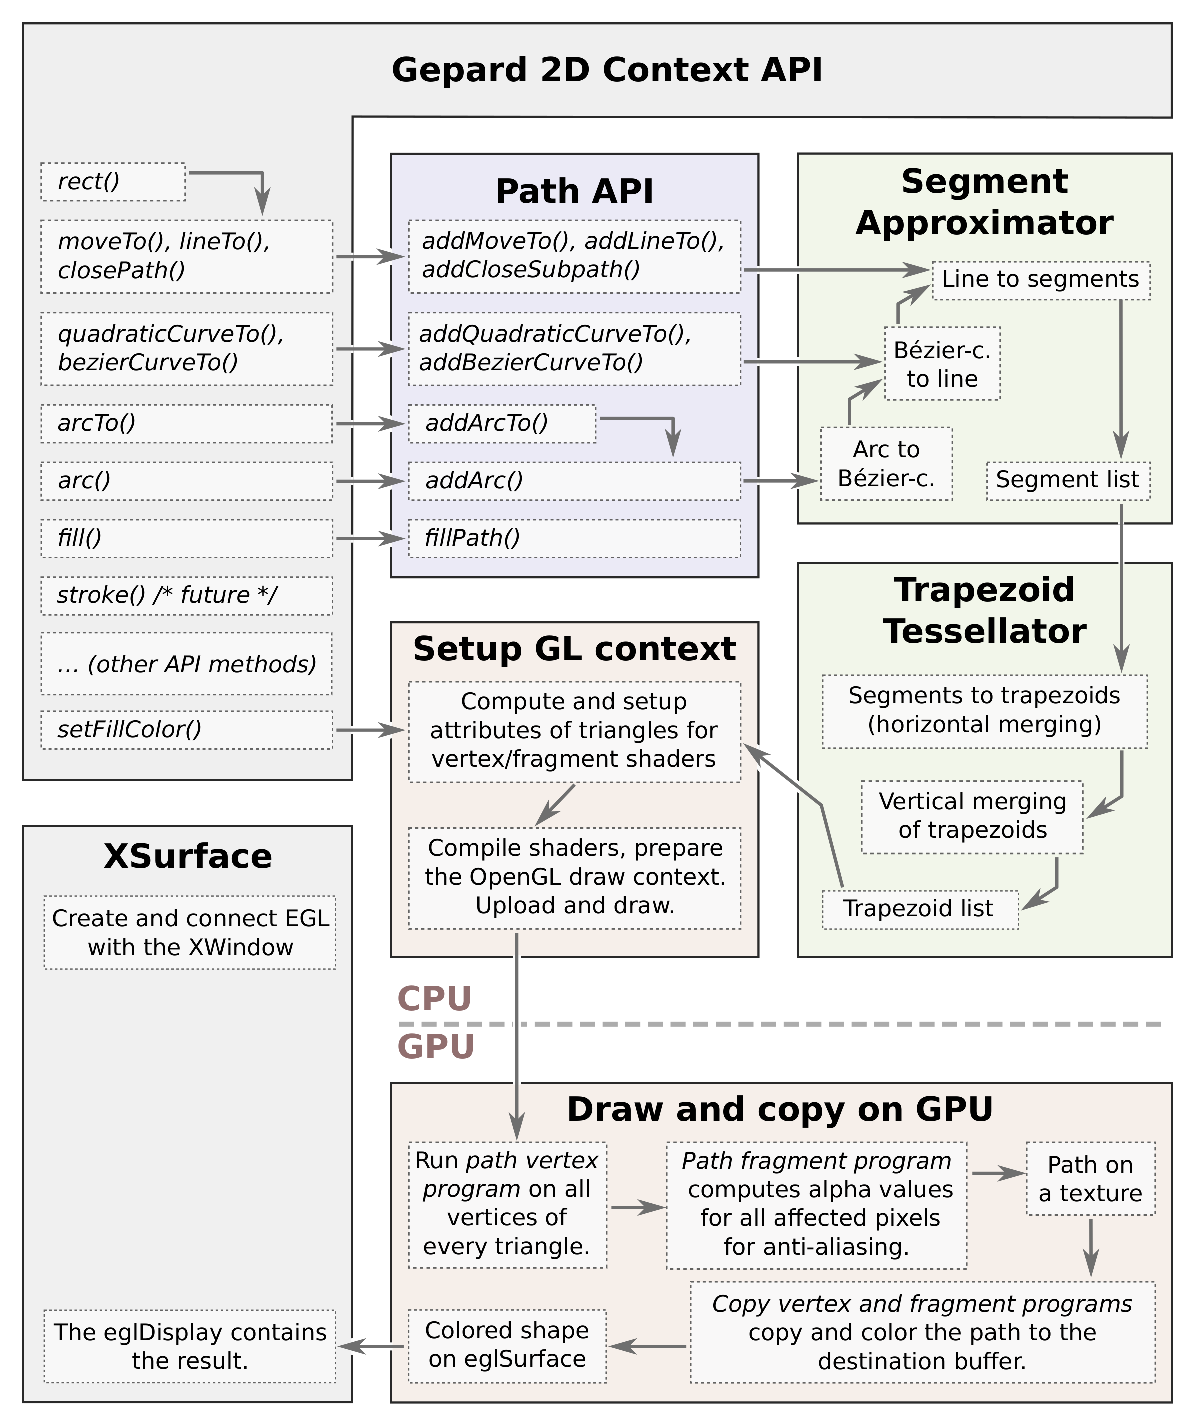
\includegraphics[scale=0.6,bb=153 355 345 595,
      clip=true]{img/built/dataflow_eps}
    \end{center}
    \caption{\label{dataflow-path-API-diagram} A belső Path API részei}
  \end{wrapfigure}

Az átalakításra azért van szükség, mert az alakzat építése közben lehetőség van
transzformációk alkalmazására, amiket az alakzatnak követnie kell. Erre szolgál
az \func{applayTransform} függvény. Gyakorlatilag a kapott
affin-transzformációval végig szorozza az addig felépített alakzat eleminek
meghatározó koordinátáit.

A bejárás lehetőségét pedig a \func{firstElement} függvény biztosítja.
Visszaadja a lista első elemének memóriacímét, amitől kezdve végig sétálhatunk
a struktúrákat tartalmazó listán. Az \func{isEmpthy} függvénnyel
lekérdezhetjük, hogy üres-e az alakzatot leíró lista. A \func{lastElement}
pedig megadja az utolsó elem memóriacímét a listában.

A már ismertetett struktúrákhoz rendre tartozik egy \func{Path} osztálybeli
függvény ami egy példányt ad a listához. Ezek a függvények bizonyos
feltételeket megvizsgálva és a szabványhoz igazodva alkalmaznak bizonyos
egyszerűsítéseket.

Az \func{addMoveToElement} függvény adja hozzá a képzeletbeli toll áthelyezését
leíró \func{MoveToElement} struktúrát. Az előírás szerint minden alakzat egy
ilyen elemmel kell kezdődjön. Ezért ez a függvény megvizsgálja, hogy az
alakzatot leíró elemek listája üres-e. Ha üres, akkor a megadott koordinátával
létrehoz egy ilyen elemet, beteszi a listába, és a listát leíró speciális
markereket (\func{firstElement}, \func{lastElement}) beállítja erre az elem
memóriacímére. Ha nem üres, és az utolsó elem a listában egy hasonló
\func{MoveToElement}, akkor értelemszerűen elégséges ennek az utolsó elemnek a
koordinátát tartalmazó adattagját módosítani az új elem értékeivel.

Az \func{addLineToElement} függvény egy egyenes vonal elemet ad a listához.
Vizsgálnia kell, hogyha még nincs elem a listában, akkor úgy kell viselkednie,
mintha egy \func{addMoveToElement} hívás történt volna. Vagyis az elem által
meghatározott (végpont) koordináta lesz az első pont. Ha nem üres a lista, és a
hozzáadni kívánt elem végpontja megegyezik az utolsó elem végpontjával, azaz
egy nulla hosszúságú vonalat kéne hozzáadni, akkor azt figyelmen kívül lehet
hagyni. Minden más esetben egy újabb \func{LineToElement}-et adunk a listához.

Az \func{addCloseSubpathElement} függvény egy alakzatot bezáró elemet ad hozzá
az listához. Ha a lista üres a függvény hívásakor, vagy az utolsó elem szintén
egy alakzatzáró, akkor a függvény mellőzi a beszúrást. A beszúrás minden
esetben egy egyenes vonalat jelent a lista legutolsó elemének végpontjától a
listában szereplő legutolsó \func{MoveToElement} pontjáig. Hogy mégis külön
struktúraként, azaz elemként kerül a listába, annak a körvonal funkcionalitása
az oka. Vagyis meg kell tudni különböztetni, hogy az adott alakzat zárt-e vagy
sem. Ami a kitöltés estében sosem kérdés, de a körvonal megrajzolásakor
kulcsfontosságú. Még akkor is fontos lehet ezt az elemet a listába szúrni, ha
az alakzat első és az utolsó pontja pont egybeesik. Ugyanis a körvonalak
végénél és a csatlakozási pontokban definiált lekerekítési stílusok
eltérhetnek, vagyis más eredményt kaphatunk a kezdő pontba húzott vagy ott be
is zárt path esetén.

Az \func{addQuadaraticCurveToElement} függvény egy másodrendű Bézier görbe
elemet add a listához. Ha a lista üres, akkor a görbe végpontját kezdő pontnak
kell tekinteni. Illetve egyszerűsítés az is, hogy ha a kontroll pont és a
végpont azonos, akkor az alakzatelem egy egyenes vonalra egyszerűsödik.

Az \func{addBezierCurveToElement} függvény egy harmadrendű Bézier görbe elemet
add a listához. Ha a lista üres, akkor a görbe végpontját kezdő pontnak kell
tekinteni.

Az \func{addArcElement} függvény egy körcikk elemet ad az alakzatot leíró
listához. Ha a lista üres, akkor kezdőpontnak a kör középpontját meghatározó
koordinátát kell választani. Ha a körcikk elfajuló, azaz nulla a sugara, vagy a
kezdő- és végszöge azonos, akkor csak egy egyenes vonalat kell húzni a kezdő
pontba, amit a kezdő szög határoz meg. Ha az utolsó elem koordinátája nem
egyenlő a körcikk kezdő pontjával, akkor szintén egyenes vonalat kell húzni a
kezdő pontba, de értelemszerűen az alakzatot leíró elemet már a listába kell
szúrni. A körcikk esetén még kisebb, a szögekkel kapcsolatos egyszerűsítéseket
lehet alkalmazni.

Az \func{addArcToElement} függvény elméletileg egy speciális körcikk elemet ad
a listához, valójában azonban ehhez a függvényhez nem tartozik külön struktúra.
Itt azért nem volt szükség külön struktúrára, mert ez a függvény által leírt
elem megadható egy egyenes vonal és egy körcikk segítségével. Ezért ez a
függvény ezt a visszavezetést tartalmazza. Arról már volt szó~\footnote{TODO:
ellenőrizni}, hogy ehhez a függvényhez egy olyan alakzatelem tartozik, ami
főleg a lekerekített alakzatok könnyebb meghatározását biztosítja. Például egy
rádiusz érték következetes használatával könnyedén definiálhatunk egy, a
sarkainál lekerekített téglalapot. Ha most ezt a téglalapot vesszük, akkor négy
ilyen alakzatelemből felépíthetjük. Ugyanakkor a valóságban négy egyenes
vonalból és négy körcikkből épül fel. Ennél az elemnél tudjuk, hogy mindig
benne van a használt pontok által meghatározott alakzatban, csupán a sarkoknál
a megadott rádiusz(ok) hatására körcikkeket kell beszúrjunk. A visszavezetés
azt kell eldöntse, hogy milyen szögtől milyen szögig terjed a körcikk, és az
előző elem végpontjából hogyan kell vonalat húzni a lekerekítést adó
körcikkhez.

    \subsection[A körvonal rajzolása]{A körvonal rajzolása}

A körvonal visszavezetését egy külön osztály (\func{StrokePathBuilder}) kezeli,
mégis a \func{Path} osztály leírásának részeként mutatjuk be. Ugyanis magának a
visszavezetést kezelő osztálynak szerkezete igen hasonló \func{Path}-éra. A
kitöltéskor egyszerűen bejárjuk az elemeket tartalmazó listát, és a
későbbiekben ismertetett módon trapézokká (végül is háromszögekké) alakítjuk az
alakzatot. A körvonal esetében egy köztes lépést alkalmazunk. Egy path
körvonala felfogható egy adott vastagságú vonalakból álló, bonyolultabb alakzat
kitöltésével. Magyarán, az eredeti path-ból képezünk egy olyan újabb
alakzatot, aminek a kitöltése az eredeti path körvonalát adja. Ezt az újabb
alakzatot továbbra is a \func{Path} osztállyal határozzuk meg. Ezért is tartjuk
indokoltnak, hogy ehhez az alfejezethez tartozóan beszéljünk róla.

Tehát a körvonal kirajzolását indukáló hívás (\emph{stroke}) hatására először a
visszavezetés történik meg. Az így kapott alakzat úgy áll elő, mint az eredeti
path vastagságát megadó \func{lineWidth} attribútum különálló részalakzatai.
Például a \func{LineToElement} elem egy téglalap alakzatként kerül az új
path-ba. Nézzük meg nagy vonalakban az egyes elemek alakzatait, illetve a
csatlakozási- és végpontoknál használt formákat.

Egy vonalat leíró elem esetén elméletileg úgy kell eljárni, hogy a vonalelemre
merőlegesen egy szakaszt helyezünk a középpontjával. A szakasz hossza a
megadott vastagsággal egyenlő. Majd a vonal mentén végigsöprünk az adott
elemen, tartva minden pontban a merőlegességet. A vásznon érintett pontok
tartoznak az adott körvonalelemhez. A gyakorlatban ez olyan három- és
négyszögek hozzáadását jelenti, amik az adott felbontás mellett lefedik az
elméleti alakzatelemet.  Például az egyenes vonalelem esetén egy azzal
párhuzamos téglalapot kell hozzáadnunk úgy, hogy a téglalap vastagsága
értelemszerűen a megadott értékkel egyenlő, hossza a vonaléval egyenlő, és a
téglalapot megadó vonalra úgy illeszkedik, hogy a vonal hosszmentén felezi a
téglalapot.

Az toll áthelyezését jelölő \func{MoveToElement}-nél ugyan nem kell különálló
formát hozzáadnunk az új alakzathoz, de lehetséges, hogy kiegészítő formákat
mégis be kell szúrjunk. Ilyen kiegészítő formák lehetnek a path végeinél a
\emph{lezárások} (\inenglish{cap}) és/vagy a köztes elemek közötti
\emph{csatlakozási pontok} (\inenglish{join}).

Az eredeti path elemeinek végpontjában (az elemek sajátosságai miatt) mindig
értelmezhetünk egy párhuzamos vektort. Egy kezdő- vagy végelem esetén
lehetséges, hogy záróformát kell illesszünk az adott elemhez. Ha kell, akkor ez
egy a vastagságot kipótoló \emph{téglalap} vagy egy abba illeszkedő
\emph{félkör} kell legyen. Ezeknek a kiegészítő formáknak az irányultságát
határozzák meg az adott pontban ismert vektorok.

Két vonal csatlakozásakor úgy kell eljárni, hogy a hézagokat töltsük fel a
meghatározott módon. Egy háromszög forma pont összekapcsolja a két elem végét.
Ha pedig szükséges, akkor egy újabb háromszög, vagy körcikk kiegészíti az
összekapcsolás pontját.

  \begin{description}[noitemsep]
    \item[Kulcsszavak] Region memory modell, line, quadratic-curve,
    cubic-curve, arc, arc-to, rect, fill, stroke, transform, translate, rotate,
    scale, skew, save, restore, color.
    \item[Becsült oldalszám] 7.
  \end{description}

  \section{Szakaszra bontás}

Ez a lelke az algoritmusomnak. Beszélnem kell az algoritmus vázáról, majd
az egyes részeket megvilágítva: mi történik a listához adott
szakaszokkal (segments), hogyan kezelem a metszéspontokat, milyen nem
ábrázolható folytonossági problémák merülhetnek fel metszések
esetén, ezeket hogyan próbáltam meg orvosolni.

  \begin{description}[noitemsep]
    \item[Kulcsszavak] Szakasz - segment, metszéspontok.
    \item[Becsült oldalszám] 6.
  \end{description}

  \section{Trapézzá alakítás}

Ebben e részben a halomra hányt szakaszokból a kitöltési metódus
alapján trapézokat hozok létre. Ezt az algoritmust is részletesen be kell
mutatnom. A trapéz építése, majd horizontális, végül vertikális
összevonásukról is kell beszélnem.

  \begin{description}[noitemsep]
    \item[Kulcsszavak] Trapéz, horizontális összevonás, vertikális összevonás.
    \item[Becsült oldalszám] 4.
  \end{description}

  \section{Rajzolás GLES2-vel}

Az rajzolás utolsó fázisa. Itt mutatom be a trapézok
háromszög-párként való kirajzolását. Hogyan gyűjtjük egybe a
háromszög-párokat, és hogyan rajzoljuk ki azokat együtt. Hogyan lesz
ebből egy alpha textúra, és azt hogyan használjuk fel színes
kirajzolásra. Itt világosítom meg, hogy miért van szükség alpha textúrára?

  \begin{description}[noitemsep]
    \item[Kulcsszavak] Batching, alpha textúra, textúrázás, színezés,
    gradiens, kivágás - clipping.
    \item[Becsült oldalszám] 4.
  \end{description}


%%%%%%%%%%%%%%%%%%%%%%%%%%%%%%%%%%%%%%%%%%%%%%%%%%%%%%%%%%%%%%%%%%%%%%
%%   Használat és eredmények                                        %%
%%%%%%%%%%%%%%%%%%%%%%%%%%%%%%%%%%%%%%%%%%%%%%%%%%%%%%%%%%%%%%%%%%%%%%

    \chapter{Használat és eredmények}
    %\addcontentsline{toc}{section}{Használat és eredmények}

    \section{Használat}

  Ez a fejezet fog szólni arról, hogy hogyan kell a \emph{libgepard.so}-t
előállítani, illetve hogyan kell használni. Bemutatok néhány egyszerű
példát.

  \begin{figure}[!htb]
    \centering
    \includegraphics[width=.95\textwidth]{img/built/erdely}
    \caption{\label{erdely} Hogy használjuk a Gepardot.}
  \end{figure}

  \begin{description}[noitemsep]
    \item[Kulcsszavak] Gepard kontext, libgepard.
    \item[Becsült oldalszám] 4.
  \end{description}

    \section{Eredmények}
    \label{Eredmények}

  Itt a lefedettséget, illetve néhány ismert rajzolóval való minőségi
összehasonlítást fogom bemutatni.

  \begin{description}[noitemsep]
    \item[Kulcsszavak] Blink, Gecko.
    \item[Becsült oldalszám] 4.
  \end{description}


%%%%%%%%%%%%%%%%%%%%%%%%%%%%%%%%%%%%%%%%%%%%%%%%%%%%%%%%%%%%%%%%%%%%%%
%%   Összefoglalás                                                  %%
%%%%%%%%%%%%%%%%%%%%%%%%%%%%%%%%%%%%%%%%%%%%%%%%%%%%%%%%%%%%%%%%%%%%%%

    \chapter{Összefoglalás}
    \addcontentsline{toc}{section}{Összefoglalás}


%%%%%%%%%%%%%%%%%%%%%%%%%%%%%%%%%%%%%%%%%%%%%%%%%%%%%%%%%%%%%%%%%%%%%%
%%   Irodalomjegyzék                                                %%
%%%%%%%%%%%%%%%%%%%%%%%%%%%%%%%%%%%%%%%%%%%%%%%%%%%%%%%%%%%%%%%%%%%%%%

    \bibliography{bib/cites}{}
    \bibliographystyle{bib/huplain}
    \addtocontents{toc}{\ }
    \addcontentsline{toc}{section}{Irodalomjegyzék}


%%%%%%%%%%%%%%%%%%%%%%%%%%%%%%%%%%%%%%%%%%%%%%%%%%%%%%%%%%%%%%%%%%%%%%
%%   Mellékletek                                                    %%
%%%%%%%%%%%%%%%%%%%%%%%%%%%%%%%%%%%%%%%%%%%%%%%%%%%%%%%%%%%%%%%%%%%%%%

    \chapter*{Mellékletek}
    \addcontentsline{toc}{section}{Mellékletek}


  \begin{figure}[!htb]
  \begin{center}
    
\includegraphics[scale=0.5]{img/built/tiger}
  \end{center}
    \caption{\label{tiger} A tiger.svg}
  \end{figure}

  \begin{figure}[!htb]
  \begin{center}
    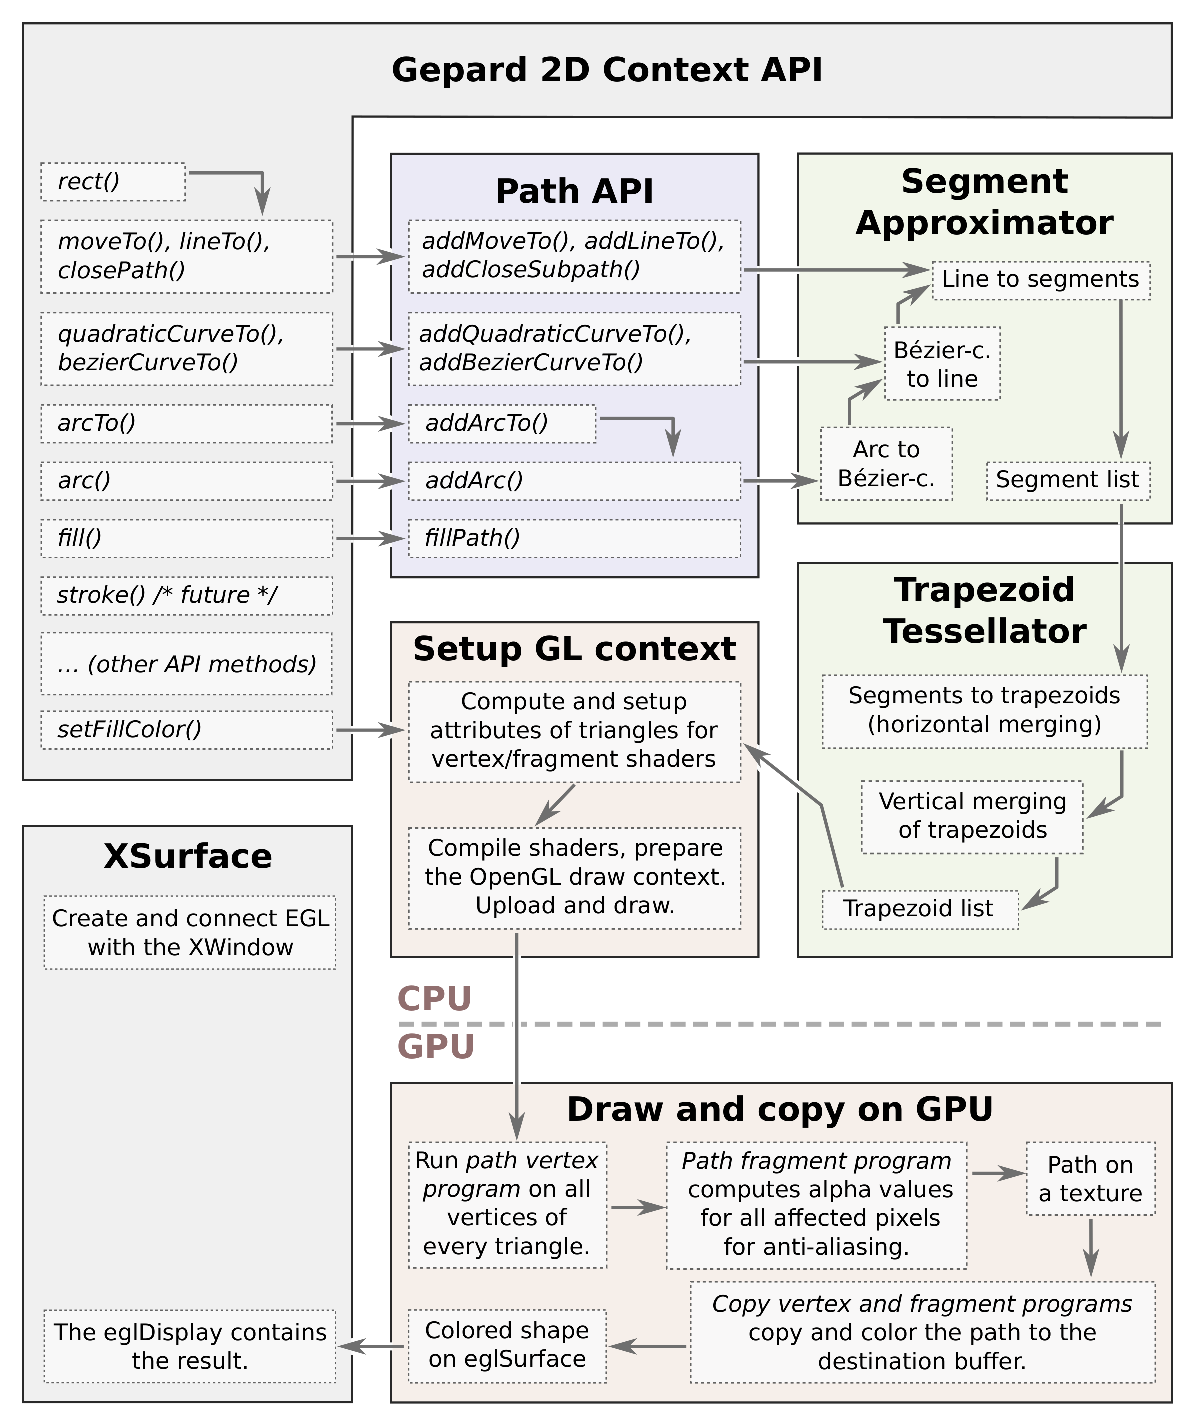
\includegraphics[scale=0.8]{img/built/dataflow_eps}
  \end{center}
    \caption{\label{dataflow_eps} A rajzolás folyamatai}
  \end{figure}


%%%%%%%%%%%%%%%%%%%%%%%%%%%%%%%%%%%%%%%%%%%%%%%%%%%%%%%%%%%%%%%%%%%%%%
%%   Nyilatkozat                                                    %%
%%%%%%%%%%%%%%%%%%%%%%%%%%%%%%%%%%%%%%%%%%%%%%%%%%%%%%%%%%%%%%%%%%%%%%

    \chapter*{Nyilatkozat}
    %Egy üres sort adunk a tartalomjegyzékhez:
    \addcontentsline{toc}{section}{Nyilatkozat}
    %\hspace{\parindent}

    % A nyilatkozat szövege más titkos és nem titkos dolgozatok esetében.
    % Csak az egyik típusú nyilatkozatnak kell a dolgozatban szerepelni
    % A pontok helyére az adatok értelemszerűen behelyettesítendők és
    % a szakdolgozat /diplomamunka szó megfelelően kiválasztandó.


    % A nyilatkozat szövege TITKOSNAK NEM MINŐSÍTETT dolgozatban a következő:
    % A pontokkal jelölt szövegrészek értelemszerűen a szövegszerkesztőben és
    % nem kézzel helyettesítendők:

    \noindent

Alulírott \makebox[4cm]{\dotfill} szakos hallgató, kijelentem, hogy a dolgozatomat a Szegedi Tudományegyetem, Informatikai Tanszékcsoport \makebox[4cm]{\dotfill} Tanszékén készítettem, \makebox[4cm]{\dotfill} diploma megszerzése érdekében.

Kijelentem, hogy a dolgozatot más szakon korábban nem védtem meg, saját munkám eredménye, és csak a hivatkozott forrásokat (szakirodalom, eszközök, stb.) használtam fel.

Tudomásul veszem, hogy szakdolgozatomat / diplomamunkámat a Szegedi Tudományegyetem Informatikai Tanszékcsoport könyvtárában, a helyben olvasható könyvek között helyezik el.

    \vspace*{2cm}

    \begin{tabular}{lc}
    Szeged, \today\
    \hspace{2cm} & \makebox[6cm]{\dotfill} \\
    & aláírás \\
    \end{tabular}


%%%%%%%%%%%%%%%%%%%%%%%%%%%%%%%%%%%%%%%%%%%%%%%%%%%%%%%%%%%%%%%%%%%%%%
%%   Köszönetnyilvánítás                                            %%
%%%%%%%%%%%%%%%%%%%%%%%%%%%%%%%%%%%%%%%%%%%%%%%%%%%%%%%%%%%%%%%%%%%%%%

    \chapter*{Köszönetnyilvánítás}
    \addcontentsline{toc}{section}{Köszönetnyilvánítás}

Ezúton szeretnék köszönetet mondani \textbf{X. Y-nak} ezért és ezért \ldots


\end{document}
